%%%%%%%%%%%%%%%%%%%%%%%%%%%%%%%%%%%%%%%%%%%%%%%%%%%%%%%%%%%%%%%%%%%%%
%% This is a (brief) model paper using the achemso class
%% The document class accepts keyval options, which should include
%% the target journal and optionally the manuscript type. 
%%%%%%%%%%%%%%%%%%%%%%%%%%%%%%%%%%%%%%%%%%%%%%%%%%%%%%%%%%%%%%%%%%%%%
\documentclass[journal=jacsat,manuscript=article]{achemso}
%\documentclass[12pt]{article}
%\usepackage[letterpaper,left=0.5in,right=0.5in,top=1.0in,bottom=1.0in]{geometry}

%%%%%%%%%%%%%%%%%%%%%%%%%%%%%%%%%%%%%%%%%%%%%%%%%%%%%%%%%%%%%%%%%%%%%
%% Place any additional packages needed here.  Only include packages
%% which are essential, to avoid problems later. Do NOT use any
%% packages which require e-TeX (for example etoolbox): the e-TeX
%% extensions are not currently available on the ACS conversion
%% servers. 
%%%%%%%%%%%%%%%%%%%%%%%%%%%%%%%%%%%%%%%%%%%%%%%%%%%%%%%%%%%%%%%%%%%%%
\usepackage[version=3]{mhchem} % Formula subscripts using \ce{}
\usepackage{siunitx} % generating degrees Celsius in the document 
\usepackage{color}
\usepackage{soul} % allows highlighting text 
\usepackage{makecell}
\usepackage{booktabs}
\usepackage{amsmath}
\usepackage{amssymb}
\usepackage{todonotes}
\usepackage{gensymb}
\usepackage{verbatim}
\usepackage{hyperref}
\hypersetup{
    colorlinks=true,
    citecolor= red,
    linkcolor=blue,
    urlcolor=blue, 
    breaklinks=true
}
\usepackage{ulem}


%%%%%%%%%%%%%%%%%%%%%%%%%%%%%%%%%%%%%%%%%%%%%%%%%%%%%%%%%%%%%%%%%%%%%
%% If issues arise when submitting your manuscript, you may want to
%% un-comment the next line.  This provides information on the
%% version of every file you have used.
%%%%%%%%%%%%%%%%%%%%%%%%%%%%%%%%%%%%%%%%%%%%%%%%%%%%%%%%%%%%%%%%%%%%%
%%\listfiles

%%%%%%%%%%%%%%%%%%%%%%%%%%%%%%%%%%%%%%%%%%%%%%%%%%%%%%%%%%%%%%%%%%%%%
%% Place any additional macros here.  Please use \newcommand* where
%% possible, and avoid layout-changing macros (which are not used
%% when typesetting).
%%%%%%%%%%%%%%%%%%%%%%%%%%%%%%%%%%%%%%%%%%%%%%%%%%%%%%%%%%%%%%%%%%%%%
\newcommand*\mycommand[1]{\texttt{\emph{#1}}}
\DeclareRobustCommand
  \Compactcdots{\mathinner{\cdotp\mkern-2mu\cdotp\mkern-2mu\cdotp}}

%%%%%%%%%%%%%%%%%%%%%%%%%%%%%%%%%%%%%%%%%%%%%%%%%%%%%%%%%%%%%%%%%%%%%
%% Meta-data block
%% ---------------
%% Each author should be given as a separate \author command.
%%
%% Corresponding authors should have an e-mail given after the author
%% name as an \email command. Phone and fax numbers can be given
%% using \phone and \fax, respectively; this information is optional.
%%
%% The affiliation of authors is given after the authors; each
%% \affiliation command applies to all preceding authors not already
%% assigned an affiliation.
%%
%% The affiliation takes an option argument for the short name.  This
%% will typically be something like "University of Somewhere".
%%
%% The \altaffiliation macro should be used for new address, etc.
%% On the other hand, \alsoaffiliation is used on a per author basis
%% when authors are associated with multiple institutions.
%%%%%%%%%%%%%%%%%%%%%%%%%%%%%%%%%%%%%%%%%%%%%%%%%%%%%%%%%%%%%%%%%%%%%
\author{Stephen P. Vicchio}
\affiliation[Clemson University]
{Department of Chemical and Biomolecular Engineering, Clemson University, Clemson, SC}
\author{Zhihengyu Chen}
\affiliation[Stony Brook University]
{Department of Chemistry, Stony Brook University, Stony Brook, NY}
\author{Karena Chapman}
\email{karena.chapman@stonybrook.edu}
\affiliation[Stony Brook University]
{Department of Chemistry, Stony Brook University, Stony Brook, NY}
\author{Rachel B. Getman}
\email{rgetman@g.clemson.edu}
\affiliation[Clemson University]
{Department of Chemical and Biomolecular Engineering, Clemson University, Clemson, SC}

%%%%%%%%%%%%%%%%%%%%%%%%%%%%%%%%%%%%%%%%%%%%%%%%%%%%%%%%%%%%%%%%%%%%%
%% The document title should be given as usual. Some journals require
%% a running title from the author: this should be supplied as an
%% optional argument to \title.
%%%%%%%%%%%%%%%%%%%%%%%%%%%%%%%%%%%%%%%%%%%%%%%%%%%%%%%%%%%%%%%%%%%%%
\title[manuscript]{
Identifying the structure and composition of \ce{Ni(II)}-hydroxo catalyst supported the NU-1000 metal-organic framework
}

%%%%%%%%%%%%%%%%%%%%%%%%%%%%%%%%%%%%%%%%%%%%%%%%%%%%%%%%%%%%%%%%%%%%%
%% Some journals require a list of abbreviations or keywords to be
%% supplied. These should be set up here, and will be printed after
%% the title and author information, if needed.
%%%%%%%%%%%%%%%%%%%%%%%%%%%%%%%%%%%%%%%%%%%%%%%%%%%%%%%%%%%%%%%%%%%%%
\abbreviations{IR,NMR,UV}
\keywords{American Chemical Society, \LaTeX}

%%%%%%%%%%%%%%%%%%%%%%%%%%%%%%%%%%%%%%%%%%%%%%%%%%%%%%%%%%%%%%%%%%%%%
%% The manuscript does not need to include \maketitle, which is
%% executed automatically.
%%%%%%%%%%%%%%%%%%%%%%%%%%%%%%%%%%%%%%%%%%%%%%%%%%%%%%%%%%%%%%%%%%%%%
\begin{document}

%%%%%%%%%%%%%%%%%%%%%%%%%%%%%%%%%%%%%%%%%%%%%%%%%%%%%%%%%%%%%%%%%%%%%
%% The "tocentry" environment can be used to create an entry for the
%% graphical table of contents. It is given here as some journals
%% require that it is printed as part of the abstract page. It will
%% be automatically moved as appropriate.
%%%%%%%%%%%%%%%%%%%%%%%%%%%%%%%%%%%%%%%%%%%%%%%%%%%%%%%%%%%%%%%%%%%%%
%\begin{tocentry}
%
%Some journals require a graphical entry for the Table of Contents.
%This should be laid out ``print ready'' so that the sizing of the
%text is correct.
%
%Inside the \texttt{tocentry} environment, the font used is %Helvetica
%8\,pt, as required by \emph{Journal of the American Chemical
%Society}.
%
%The surrounding frame is 9\,cm by 3.5\,cm, which is the maximum
%permitted for  \emph{Journal of the American Chemical Society}
%graphical table of content entries. The box will not resize if the
%content is too big: instead it will overflow the edge of the box.
%
%This box and the associated title will always be printed on a
%separate page at the end of the document.
%
%\end{tocentry}

%%%%%%%%%%%%%%%%%%%%%%%%%%%%%%%%%%%%%%%%%%%%%%%%%%%%%%%%%%%%%%%%%%%%%
%% The abstract environment will automatically gobble the contents
%% if an abstract is not used by the target journal.
%%%%%%%%%%%%%%%%%%%%%%%%%%%%%%%%%%%%%%%%%%%%%%%%%%%%%%%%%%%%%%%%%%%%%
\begin{abstract}
Metal-organic frameworks (MOFs) provide an excellent platform for supporting 3d transition metal complexes. Despite being catalytically active for gas-to-liquid transformations of natural gas, open questions about the exact structure of the catalytically-active state of the metal complex inhibit our ability to rationally design these catalysts. These supported metal cation complexes exhibit structures changes that affect catalytic performance when exposed to different reaction environments (such as an increase in temperature and exposure to \ce{H2} gas). Therefore, to reach their full-potential as catalytic materials, fundamental insights into the relationship between reaction environment, structure, and performance are required. We use a combined density functional theory (DFT) and \textit{ab initio} thermodynamic analysis to determine the structure and composition of a tetranuclear \ce{Ni} metal complex supported on NU-1000. Here we show that the lowest energy structural and compositional arrangement of the \ce{Ni} cluster is highly sensitive to reaction conditions (temperature, \ce{H2O} partial pressure, and \ce{H2} partial pressure) using phase diagrams, which reveal the thermodynamic landscape of the \ce{Ni} cluster. We compare the local atomic structures of our thermodynamic models to experimentally local structural information obtained by differential pair distribution functions (dPDFs). By comparing the local structural information for model structures and experimental data, specifically the \ce{Ni-O}, \ce{Ni{\Compactcdots}Ni}, and \ce{Ni{\Compactcdots}Zr} atomic distances, we demonstrate the importance of \ce{H2O} within the \ce{Ni} metal complex active site in maintaining a high \ce{Ni} coordination. We find highly coordinated structures show much better agreement to the experimental data. Our computational modeling demonstrates how the catalyst structure is controlled by temperature and partial pressure. The findings establish thermodynamically relevant models that require further computational catalytic investigations as well as showcasing how to tune structures using different reaction conditions.
\end{abstract}

%%%%%%%%%%%%%%%%%%%%%%%%%%%%%%%%%%%%%%%%%%%%%%%%%%%%%%%%%%%%%%%%%%%%%
%% Start the main part of the manuscript here.
%%%%%%%%%%%%%%%%%%%%%%%%%%%%%%%%%%%%%%%%%%%%%%%%%%%%%%%%%%%%%%%%%%%%%

\section{Introduction}

%Traditionally, chemical reaction on heterogeneous catalysts occurs at the surface of a solid catalyst with a small number of metal atoms participating in the reaction. Unlike in homogeneous catalysts, which feature well-defined isolated active sites and high metal utilization, the exact geometric and electronic nature of a heterogeneous catalyst active site is often unknown or challenging to elucidate.

% These newly envisioned heterogeneous catalytic materials are called

% Recent scientific advancements address limitations in heterogeneous catalysts by designing catalysts with that

Single-site heterogeneous catalysts (SSHCs), i.e., which contain uniform active sites featuring one or more atoms that are spatially and electronically isolated from each other,\cite{Rogge2017} mimic the isolated active sites of homogeneous catalysts while remaining anchored to solid supports.\cite{Hlatky2000,Kaiser2020}  .\cite{Thomas2005,Wasson2019} Supports for SSHCs include metal-organic frameworks (MOFs),\cite{Zheng2019,AbdelMageed2019,Huang2019} .\cite{Cui2018,Noh2016,Li2017,Song2019,Nguyen2015,Hackler2020} covalent-organic frameworks (COFs),\cite{Zhong2019,Romero-Muniz2020}, zeolites,\cite{Mao2016, Kistler2014} and metal\cite{Patel2019,Pei2017,Qian2012,Jiao2019}  and metal oxide surfaces.\cite{Bo2019,Riley2018,Tang2019}The atomically dispersed atoms are often 3d transition metals,\cite{Manna2016,Beyzavi2015} with the solid support providing a means to improved metal utilization and more well-defined active site structures.\cite{Qiao2011,Cui2017,Yang2013} The metal atoms are anchored to the support by ligands... Hence, the active site structure for any given SSHC is unique, which makes SSHCs appealing for carrying out challenging chemistries, i.e., by capitalizing on the diversity and tunability of SSHCs as a means to potentially improve catalytic activity and selectivity.

The downside to this uniqueness is that it complicates catalyst design, since the patterns of behavior that are more common with traditional bulk metal catalysts are not present. For example, ... This is further complicated by the influence of reaction conditions. Unlike for bulk metal catalysts, where the influence of reaction conditions on the catalyst surface properties are well known,\cite{Getman2008,Piccinin2017,Zuo2016,Bray2015} for SSHCs, reaction conditions additionally induce changes in coordinating ligands and steric environments that influence the mechanism\cite{Kim2015,Redfern2018,Mian2020,Shabbir2020} and do not necessarily follow periodic trends. Given catalyst structure drives catalyst function, there is a growing need to understand how the environmental conditions transforms the active site structure under a variety of conditions.\cite{Tang2019} The unambiguous determination of SSHC active sites remains an ongoing challenge, with rational catalyst design inhibited by difficulties in determining the precise active site.

%difficulties in determining the precise active site structure poise significant limitations in catalyst design. 

% The structure of the active site on these various supports is defined by the dispersed metal species, coordinating ligands, and steric environment with these factors contributing to the reactivity and selectivity of the catalyst. The 

Environmental conditions have a profound effect on SSHC active site structure. Responsive structural transformations for SSHCs include sintering of the metal atoms,\cite{Mian2020,Halder2020} dispersion of the metal atoms,\cite{Jones2016} and changes in the local coordination environment.\cite{Ye2017,Daelman2019} For example, \citeauthor{DeRita2019} demonstrates that local coordination of \ce{Pt} atoms deposited on \ce{TiO2} nanoparticles evolve in response to environmental conditions and elucidates how these structural changes strongly influence the chemical reactivity for \ce{CO} oxidation.\cite{DeRita2019} Similarly, environmental conditions activate the metal complex by altering the local coordination by manipulating the ligands present for on a Nickel(II)-hydroxo supported metal complex in a MOFs.\cite{Li2016sintering,Ye2017} Conversely, environmental conditions can also fundamentally alter the active site structure from a Copper(II)-hydroxo SSHC to encapsulated nanoparticles in MOFs.\cite{Halder2020,Mian2020} Predicting how environmental conditions alter any SSHC is non-trivial, and depends on both the type of SSHC and the support. The heterogeneity of SSHCs and their supports makes characterizing the active site structure challenging. Systematically addressing how the local coordination environment changes in responses to variations in environmental conditions is essential when determining structure-function relationships for SSHCs regardless of the support. 

% Since the local coordination environment has a strong influence on catalytic performance, learning the precise SSHC active site structure, which is already challenging, is exacerbated by the influence of environmental conditions. 

% Combined experimental and computational approaches address SSHC active site characterization questions when exposed to different environmental conditions.

% , with porous materials containing complex variations

In this work, we attempt to learn the structure of single site nickel catalysts supported in MOFs. Specifically, we investigate a \ce{Ni(II)} catalyst supported on the MOF NU-1000.; specifically, we investigate the \ce{Ni}-AIM catalyst \citeauthor{PlateroPrats2017}\cite{PlateroPrats2017}. For SSHCs supported on MOFs, \hl{EXPLANATION NEEDED} first there was a hypothesis about single Ni hydrides and then something came along and suggested that was wrong, so the new hypothesis shifted to some other structure I don't remember... We know that structure isn't perfectly correct, either and state why. I.e., elaborate a bit on the history here. This ambiguity is further complicated by temperature and gas phase species.\cite{PlateroPrats2017b,Rimoldi2017,Ikuno2017} For example, under \ce{H2} gas (i.e., reducing conditions), the local coordination of the \ce{Ni(II)} metal complex is thought to contain a Nickel hydride (\ce{Ni-H})\cite{Shabbir2020} formed via the removal of coordinating \ce{H2O} ligands.\cite{Li2016sintering,Shabbir2020} OTHER EXAMPLES? Given the sensitivity of the ligand environment to gas phase conditions and the fact that the precise structure and ligand environment is still unknown, we explore the local coordination of a \ce{Ni(II)} metal complex supported on the NU-1000 MOF under different gas phase atmospheres. We specifically explore \ce{H2} gas because ... (reducing conditions)  Using \textit{ab initio} thermodynamic analysis and differential pair distribution functions (dPDF) analysis, local structural information is observed. We find ... Our results provide insights into the local coordination of the Nickel metal complex, including the evolution of \ce{OH}-ligands and the role of \ce{H2O} within the active site, to establish more appropriate molecular models.

% , a porous crystalline material formed from inorganic nodes interconnected by organic linkers,\cite{Furukawa2013,Li1999} are commonly used to support 3d transition metal complexes to form SSHCs.

% and coordinating ligands (e.g., \ce{OH}/\ce{OH2}), generate the active site structure. 

% Herein, we call the experimental \ce{Ni(II)} metal complex supported on the NU-1000 as \ce{Ni}-AIM (\underline{A}tomic Layer Deposition \underline{i}n \underline{M}OFs) thereby adopting the same notation as \citeauthor{PlateroPrats2017}\cite{PlateroPrats2017}

% from thermodynamically-relevant \ce{Ni4}-cluster models are compared directly to experimental Nickel clusters under similar environmental conditions

%%%%%%%%%%%%%%%%%%%%%%%%%%%%%%%%%%%%%%%%%%%%%%%%%%%%%%%%%%%%%%%%%%%%%
%% Methodology
%%%%%%%%%%%%%%%%%%%%%%%%%%%%%%%%%%%%%%%%%%%%%%%%%%%%%%%%%%%%%%%%%%%%%
\section{Methodology}

\begin{figure}[H]
    \centering
    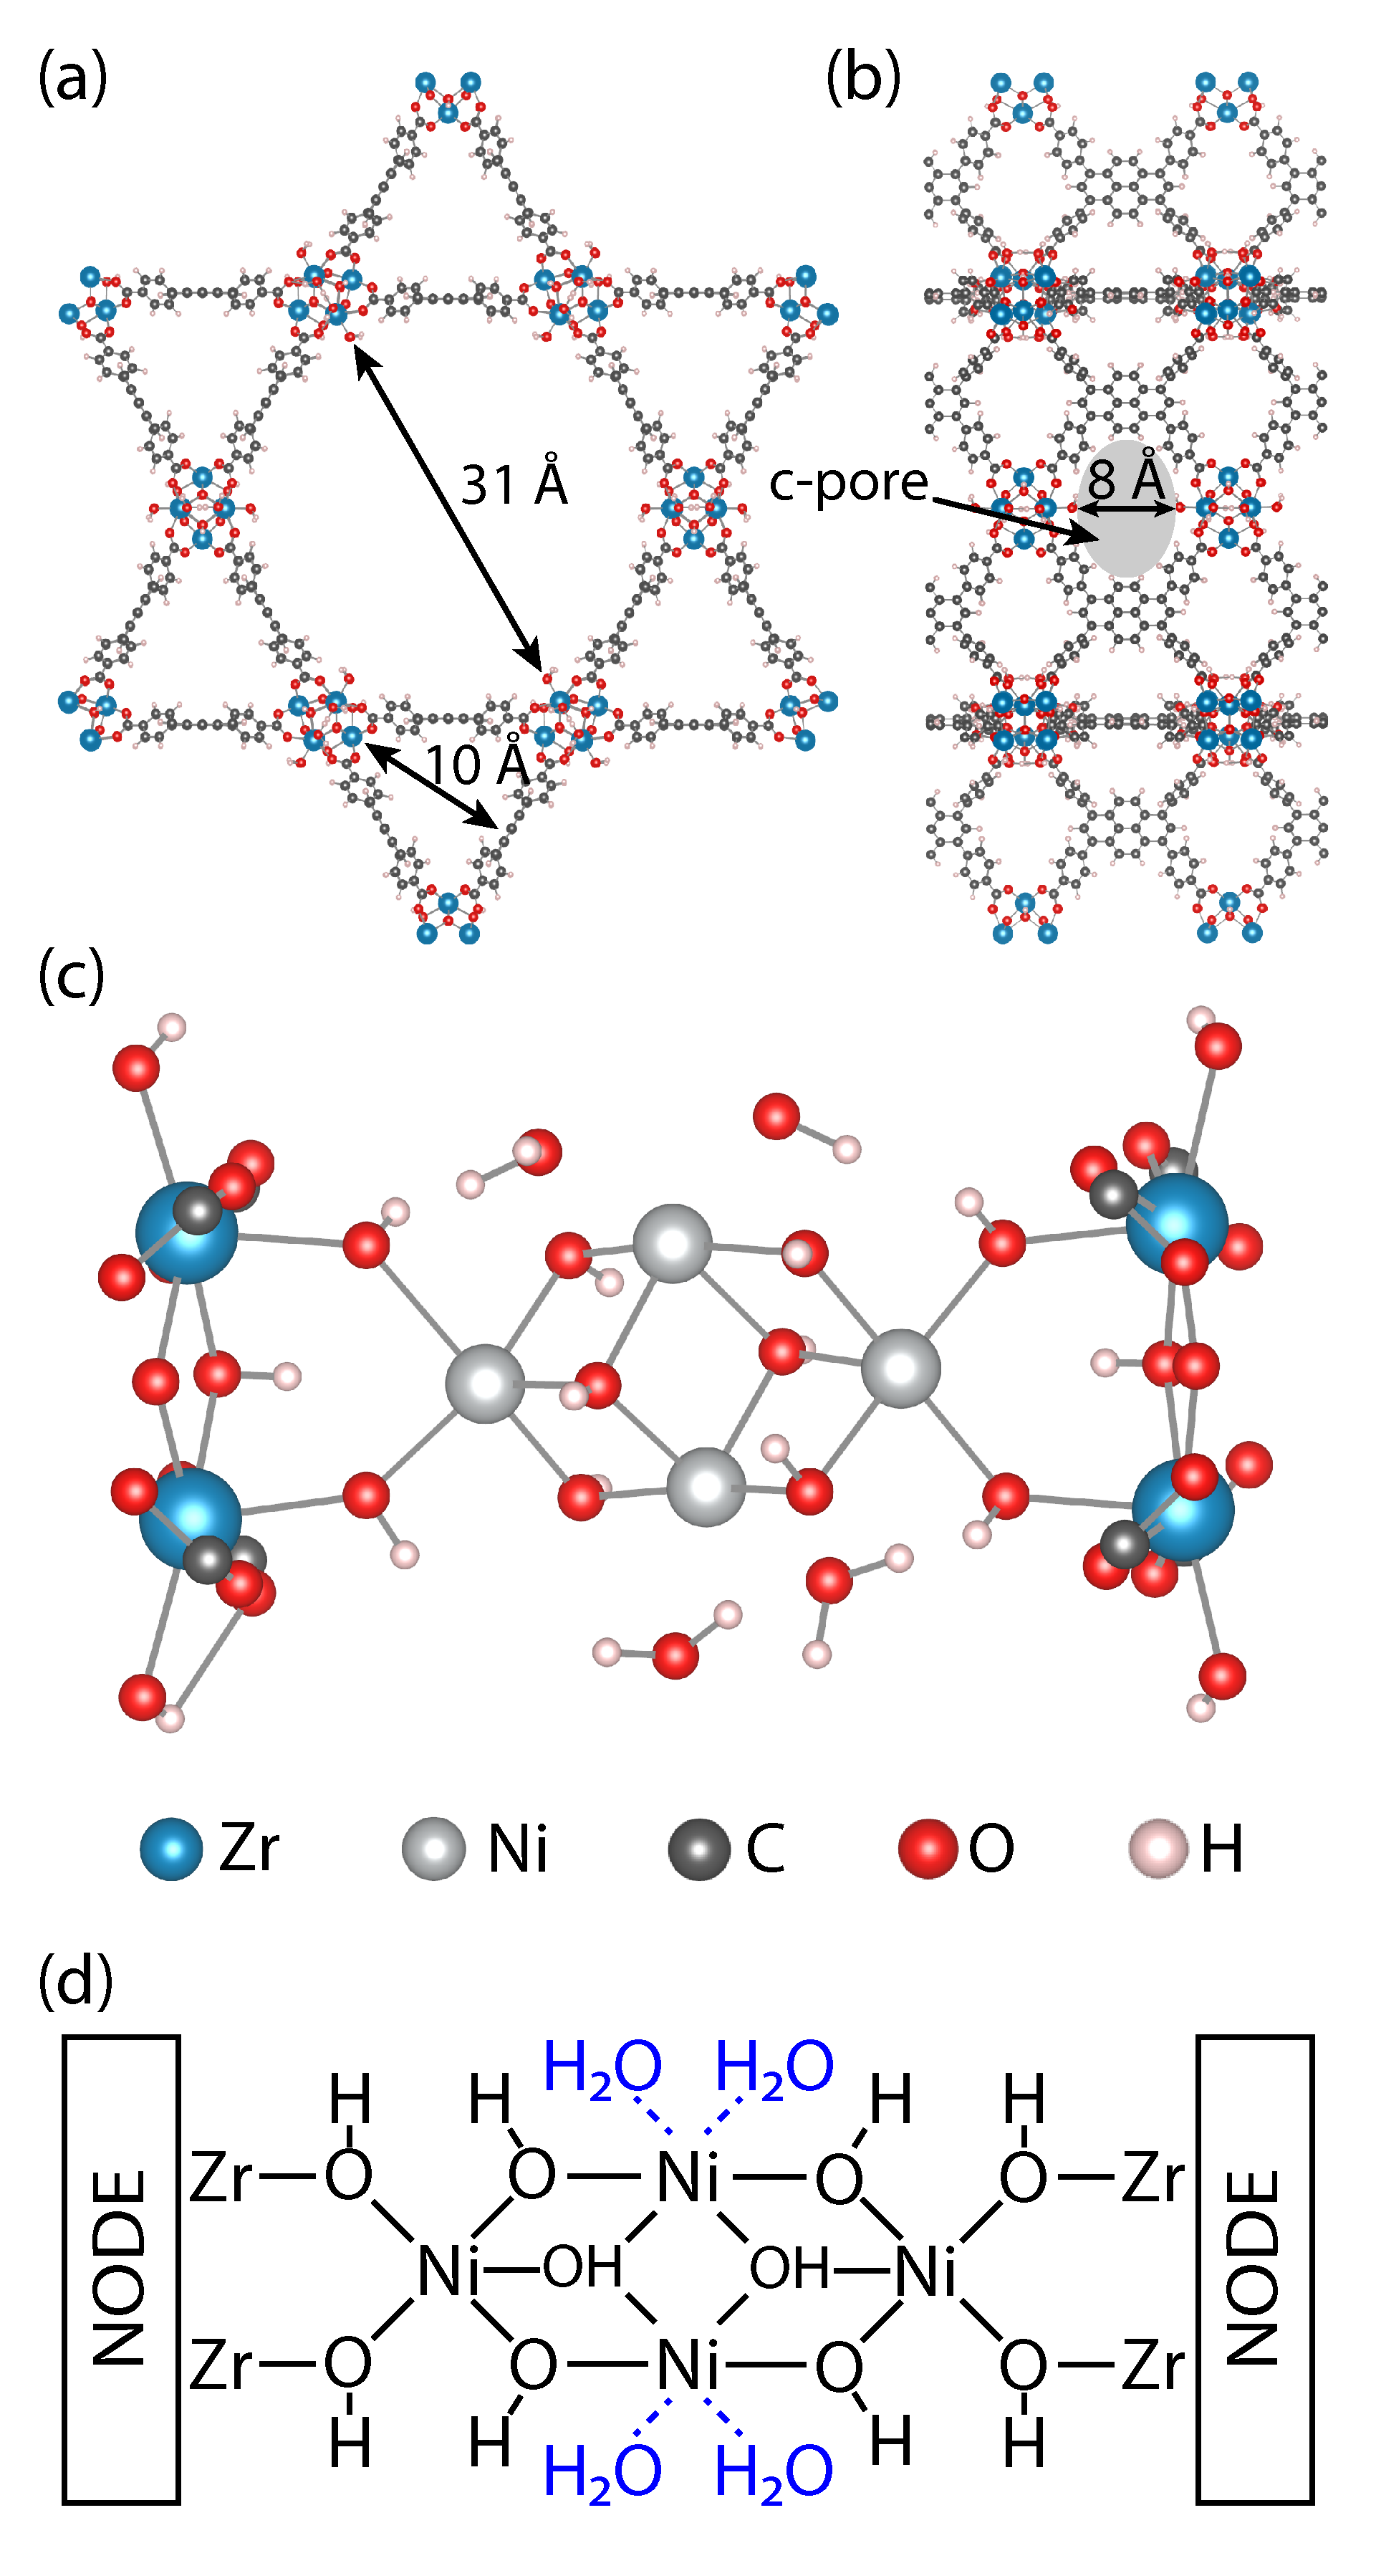
\includegraphics[width=3.0in]{zi-images/00-General-Graphics/2021-figure-MOF-structure.png}
    \caption{
    The structure of NU-1000 shown along the (a) c-axis and the (b) a-axis with the location of the metal complex location highlighted by the gray oval in (b). The gray oval spans the c-pore of NU-1000 (\~10 {\AA}). Different variations of the \ce{Ni4}-cluster are shown in (c) and (d) with the node of the MOF framework truncated from the renderings. All adsorbed \ce{H2O} molecules are outlined in blue. 
    }
    \label{fig:Ni-MOF-model}
\end{figure}

\subsection{Computational Details}

\subsubsection{Catalyst Models}

NU-1000 (Figure~\ref{fig:Ni-MOF-model}a) comprises zirconium oxide (\ce{Zr6(\mu_{3}-O)4(\mu_{3}-OH)4(H2O)4(OH)4}) nodes connected by pyrene linker molecules. The resulting crystal structure contains large hexagonal channels (31 {\AA}), triangular channels (10 {\AA}), and small pores (8 {\AA}) as shown in Figures~\ref{fig:Ni-MOF-model}a and~\ref{fig:Ni-MOF-model}b. DFT-optimized unit cell parameters are $a=b=40.611$ {\AA}, $c=15.990$ {\AA}, $\alpha=\beta=\ang{90}$, and $\gamma=\ang{60}$, in agreement with prior work.\cite{PlateroPrats2017} \ce{Ni(II)} catalyst models comprise between two and four \ce{Ni(II)} cations (denoted as \ce{Ni^{*}}). The choice to use a maximum of four \ce{Ni^{*}} is based off prior work, with \citeauthor{PlateroPrats2017} revealing the \ce{Ni(II)} cluster most likely consists of four \ce{Ni(II)} atoms from difference envelope density (DED) analysis\cite{PlateroPrats2017}. Catalyst models are constructed within the the NU-1000 ``c-pore," (Figure~\ref{fig:Ni-MOF-model}b) following prior work.\cite{PlateroPrats2017} Here, they attach to NU-1000 by replacing protons on the NU-1000 \ce{Zr} nodes;CITE structures with three and four \ce{Ni} cations can bridge adjacent NU-1000 nodes,\cite{Ye2017} as shown in Figures~\ref{fig:Ni-MOF-model} (c) and (d). Catalyst models adopt a variety of ligand environments that include hydroxyl (\ce{OH^{*}}), water (\ce{H2O^{*}}), and hydride (\ce{H^{*}}) ligands. In all, we evaluated \textbf{\color{red}XXX} structures; \textbf{\color{red}the full library can be accessed on our GitHub page.} 

% (from a \ce{OH/OH2} pair) thereby giving NU-1000 a net formal charge of $-$2 and the \ce{Ni(II)} catalyst model a net formal charge of $+$2.

\subsubsection{\textit{ab initio} Thermodynamics Modeling}

The influence of temperature and gas phase composition is explored using \textit{ab initio} thermodynamic analysis. In this method, a phase diagram is constructed to report the structures that minimize the free energy in equilibrium with temperatures and pressures in a gas phase reservoir.\cite{Reuter2003,Reuter2004,Grundner2015,Paolucci2016,Li2016,Getman2008,Mandal2020,Zuo2016,Tang2019} The free energy of each structure is calculated as
\begin{equation}
    \begin{split}
        \Delta F^{(2)}(V,T,\mu_{\text{H}^{*}},\mu_{\text{OH}^{*}},N_{\text{Ni}^{*}})  
        & = \Delta F(V,T,N_{\text{H}^{*}},N_{\text{OH}^{*}},N_{\text{Ni}^{*}}) - (\mu_{\text{H}^{*}})(\Delta N_{\text{H}^{*}}) \\ 
        & - (\mu_{\text{OH}^{*}})(\Delta N_{\text{OH}^{*}})  \\ 
    \end{split}
    \label{eq:free-energy-trans}
\end{equation}
where $F$ is the Helmholtz free energy, $V$ is volume, $T$ is temperature, $\mu$ is chemical potential, and $N$ is the number of each type of ligand. The (2) superscript on $F^{(2)}$ indicates the second Legendre transform of $F$, i.e., of $N_{\ce{H}^{*}}$ and $N_{\ce{OH}^{*}}$ to $\mu_{\ce{H}^{*}}$ and $\mu_{\ce{OH}^{*}}$, respectively. $F$ for a solid is usually set equal to $E^\text{elec} + E^\text{ZP} + F^\text{vib}$, where $E^\text{elec}$ is the electronic energy calculated with DFT, $E^\text{ZP}$ is the zero point vibrational energy, and $F^\text{vib}$ is the temperature dependent vibrational free energy. We find that $E^\text{ZP} + F^\text{vib}$ contribute negligibly to $F$ (see Supporting Information) and hence approximate $F \approx E^\text{DFT}$. The $\Delta$'s in Eq.~\ref{eq:free-energy-trans} indicate quantities taken relative to a reference structure. The reference structure is defined as a \ce{Ni4(OH)6} cluster with four \ce{H2O} ligands (see supporting information Figure SXXX). To simulate reaction conditions commensurate with catalytic hydrogenation, free energies are calculated assuming equilibrium with a \ce{H2} reservoir. Further, since H addition to \ce{OH^{*}} ligands creates \ce{H2O^{*}} ligands which can theoretically desorb, the structure is also assumed to be in equilibrium with an \ce{H2O} reservoir. Following these assumptions, $\mu_{\ce{H}^{*}} = 1/2 \mu_{\ce{H}_2(\text{g})}$, $\mu_{\ce{H2O}^{*}} = \mu_{\ce{H2O}(\text{g})}$, and $\mu_{\text{OH}^{*}} = \mu_{\text{H}_2\text{O}^{*}} - \mu_{\text{H}^{*}}$. By definition, $\mu$ are functions of $T$ and $P$. Assuming ideal gas conditions, $\mu_{\text{H}_2(\text{g})}$ is\cite{Reuter2003,Reuter2004,Grundner2015,Paolucci2016,Li2016,Getman2008,Mandal2020}   
\begin{equation}
    \mu_{\text{H}_{2}(\text{g})}(T,P_{\text{H}_{2}}) = E^\text{elec}_{\text{H}_{2}} + E^\text{ZP}_{\text{H}_{2}} + \left[ G_{\text{H}_{2}}(T,P^{o}) - G_{\text{H}_{2}}(0~\text{K},P^{o}) + RT \ln{\left( \frac{P_{\text{H}_{2}}}{P^{o}} \right)} \right]  
    \label{eq:chemicalpotentialrel}
\end{equation}
where $G$ is the Gibbs free energy, $P$ is partial pressure, and $P^{o}$ is the standard pressure (1 bar). We calculate values of $G$ using the NASA Polynomials\cite{Mcbride1993} in the pMuTT\cite{LYM2019106864} Python package. $G(0~\text{K},P^{o})$ is approximated as $G(10~\text{K},P^{o})$ and obtained by extrapolating the NASA Polynomials, following prior work.\cite{Getman2008,Li2016} $\mu_{\text{H}_2\text{O}(\text{g})}$ is computed analogously. Phase diagrams could be constructed in three dimensions, i.e., as functions of $T$, $P_{\text{\ce{H2}}}$, and $P_{\text{\ce{H2O}}}$. However, since \ce{H2O} is not typically added in hydrogenation reactions, in our analysis, we construct two dimensional phase diagrams as functions of $T$ and $P_{\text{\ce{H2}}}$. These phase diagrams are constructed at constant $P_{\text{\ce{H2O}}}$ of $10^{-1}$ bar. This value was chosen since it leads to structures with \ce{Ni^*} coordination numbers that are commensurate with experimental observation (see Section \hl{XXX}). To test the influence of temperature and gas phase composition on the \ce{Ni^*} coordination number, we additionally investigate scenarios where \ce{Ni^*} are removed from the structure, i.e., by aggregating to form Ni metal. In these circumstances, we take an additional Legendre transformation of $F^{(2)}$ into $F^{(3)}$ by transforming $N_{\ce{Ni^*}}$ into $\mu_{\ce{Ni^*}}$, where $\mu_{\text{Ni}^{*}} = \mu_{\text{Ni}(\text{s})}$ and $\mu_{\text{Ni}(\text{s})} = E^\text{elec}_\text{Ni(s)}$, following prior work.\cite{Grundner2015} A full description of how $E_\text{Ni(s)}$ is calculated is provided in Supporting Information. Further details about the thermodynamic modeling approach as well as sensitivity analyses for the various modeling decisions are provided in \hl{supporting information}. The Supporting Information also includes phase diagrams simulated at lower pressures of \ce{H2O}.

%Phase diagrams constructed at $P_{\text{\ce{H2O}}} < 10^{-1}$~bar are provided in Supporting Information.

\subsubsection{Density Functional Theory Calculations}

Electronic energies are calculated using the CP2K software package.\cite{Hutter2014} The exchange correlation energy is calculated with the PBE functional\cite{Perdew1996} and corrected using damped D3 dispersion corrections formulated by \citeauthor{Grimme2010}\cite{Grimme2010} The DZVP-MOLOPT basis set is used to model the valance electrons, and the Goedecker pseudopotentials\cite{Goedecker1996} are used to model the core electrons. The plane wave cutoff energy is 360 Ry. The Unrestricted Kohn-Sham (UKS) method is employed given the open shell natures of the \ce{Ni} ions. For example, a single \ce{Ni(II)} ion can adopt either a singlet or triplet state; therefore, clusters with four \ce{Ni} ions can adopt singlet, triplet, quintet, septet, or nonet states. We consider all possible spin states for \ce{Ni} for each catalyst composition.\cite{Shabbir2020,Ye2017,Bernales2016,Mandal2020b} Any spin state exhibiting spin contamination is not considered in \textit{ab initio} thermodynamic modeling (see supporting information for more details). The final values of $E$ used in \textit{ab initio} thermodynamic modeling are obtained from geometry relaxations where all atoms in the periodic unit cell are allowed to relax. A sample input file for the CP2K calculations is provided in Supporting Information. Additionally, full descriptions of how $E_{\text{H}_2}$ and $E_{\text{H}_2\text{O}}$ are calculated are provided in Supporting Information.

\subsection{Experimental Details}

The pair distribution function (PDF), G(r), represents the local structure as a histogram atom-atom distances in the material weighted by the scattering power of the atoms involved. While the measured PDF reflects all atom-atom distances within the material, by deriving a differential PDF (dPDF), where the PDF measured for NU-1000 is subtracted from the PDF measured for the Ni-complex containing Ni-NU-1000, we analytically isolate the atom-atom distances that define the \ce{Ni} cluster and its interaction with NU-1000 support. Thus the dPDF includes the interatomic distances  within the cluster (\ce{Ni{\Compactcdots}Ni}, \ce{Ni-O}, \ce{O{\Compactcdots}O} atom pairs) and between the cluster and the MOF (\ce{Ni{\Compactcdots}Zr} and \ce{Ni{\Compactcdots}O}) with atom pairs not directly bonded to each other receiving the ``${\Compactcdots}$" notation. PDFs of the computed structural models were simulated within PDFgui using typical values of instrument and atomic displacement parameters for such materials. Given the lower scattering contribution from the \ce{O} atoms compared to \ce{Ni} atoms, \ce{O{\Compactcdots}O} pairs have very low contribution to the measured data and were not calculated. The simulated PDFs were evaluated for their correspondence to the experimental data over XYZ {\AA} range. The experimental details of the PDF measurements are described elsewhere in detail.\cite{PlateroPrats2017} The tetranuclear Nickel cluster exposed to \ce{H2} (3.5\% in \ce{He}) at 200 \degree C for 2 hours and then cooled to 50 \degree C in \ce{H2} for measurement.\cite{PlateroPrats2017} Powder X-ray diffraction (XRD) and total scattering data suitable for PDF analysis were collected at 50 \degree C in \ce{H2}. The dPDFs provide structural insights into the cluster by revealing key interatomic distances with peaks indicating the distance between different atoms. First coordination sphere distances are reported using a line (e.g., \ce{Ni-O}) while second coordination sphere distances are reported using dots (e.g., \ce{Ni{\Compactcdots}Ni} and \ce{Ni{\Compactcdots}Zr}).

%%%%%%%%%%%%%%%%%%%%%%%%%%%%%%%%%%%%%%%%%%%%%%%%%%%%%%%%%%%%%%%%%%%%%
%% Results
%%%%%%%%%%%%%%%%%%%%%%%%%%%%%%%%%%%%%%%%%%%%%%%%%%%%%%%%%%%%%%%%%%%%%

\section{Results}
To provide insight into the types of structures and compositions that could be observed experimentally, phase diagrams were constructed for $P_{\text{\ce{H2}}}$ spanning from ultrahigh vacuum to ambient and temperatures spanning from 20$^\circ$C to 300$^\circ$C in Figure~\ref{fig:phase_diagram_Ni_combined}.  Specifically, Figure~\ref{fig:phase_diagram_Ni_combined} (a) plots the thermodynamically preferred structures with $2 \le N_{\ce{Ni^*}} \le 4$ while Figure~\ref{fig:phase_diagram_Ni_combined} (b) plots structures with $N_{\ce{Ni^*}} = 4$. The structures represented on the phase diagrams are hence those that minimize $F^{(2)}$ (Figure~\ref{fig:phase_diagram_Ni_combined}b) or $F^{(3)}$ (Figure~\ref{fig:phase_diagram_Ni_combined}a) at the given conditions. Depictions illustrating the compositions and roughly the structures of these structures are shown in Figure~\ref{fig:Ni-structure-diagram}. Full structural information is provided ... 

The structures on the phase diagrams exhibit different compositions and including $\ce{OH^{*}}$, $\ce{H2O^{*}}$, and $\ce{H^{*}}$ ligands coordinated to the \ce{Ni} atoms. At low \hl{H2 partial pressures} and temperatures below 100 \degree C, the most energetically preferred structure in both Figures~\ref{fig:phase_diagram_Ni_combined} (a) and (b) is 4-\ce{Ni4(OH)4}. In this structure, the first coordination spheres of the \ce{Ni} atoms comprise $\ce{OH^{*}}$ and $\ce{H2O^{*}}$ ligands, with OH forming links between Ni ions and H2O binding on the ``open" sites of the Ni ions in the center of the chain. This suggests that at low \hl{H2 partial pressures} the thermodynamics of the cluster aren't sensitive to the \ce{Ni} composition. 

With increasing \hl{H2 partial pressures}, Figures 2a and 2b yield different thermodynamic minimum. Specifically, considering the phase diagram in Figure~\ref{fig:phase_diagram_Ni_combined} (a), at temperatures above 100 \degree C, increasing $P_{\ce{H2}}$ results in a loss of \ce{Ni^*}. This occurs since increasing \ce{H2} partial pressure results in conversion of $\ce{OH^{*}}$ to $\ce{H2O^{*}}$; the $\ce{H2O^{*}}$ that form can then desorb, resulting in a loss of ligands. For example, going from structure 4 to 5 and 5 to 6 in Figure 2a... briefly describe what happens, e.g., the OH ligands that connect Ni ions to each other are hydrogenated; and it is more thermodynamically preferable for the resulting water ligands desorb and the coordinated Ni to agglomerate than for the H2O ligand to remain in the structure. When this happens, the Ni cations are destabilized and hence attempt to minimize their free energies via aggregation. As a result, the dominant structure in Figure~\ref{fig:phase_diagram_Ni_combined} (a), structure 6-\ce{Ni2(H)2} (lilac), comprises isolated nickel hydride species; interestingly, such species have been previously suggested as the active sites in catalytic ethylene hydrogenation\cite{Li2016sintering,Shabbir2020} and ethylene dimerization.\cite{Ye2017} In contrast, the dominant structure in Figure~\ref{fig:phase_diagram_Ni_combined} (b) is structure 4 cite if previously identified; this structure features four Ni ions linked by hydroxyl ligands; however, the Ni in the center of the chain are undercoordinated due to loss of OH ligands via hydrogenation. In Figure 2b, lowering lowering of the temperature below 50\degrees C recovers the H2O ligands, first forming adsorbed H2O that turns into a chain of hydrogen bonded H2O molecules below 40\degrees C.

% The combined phase diagram figures
\begin{figure}[H]
    \centering
    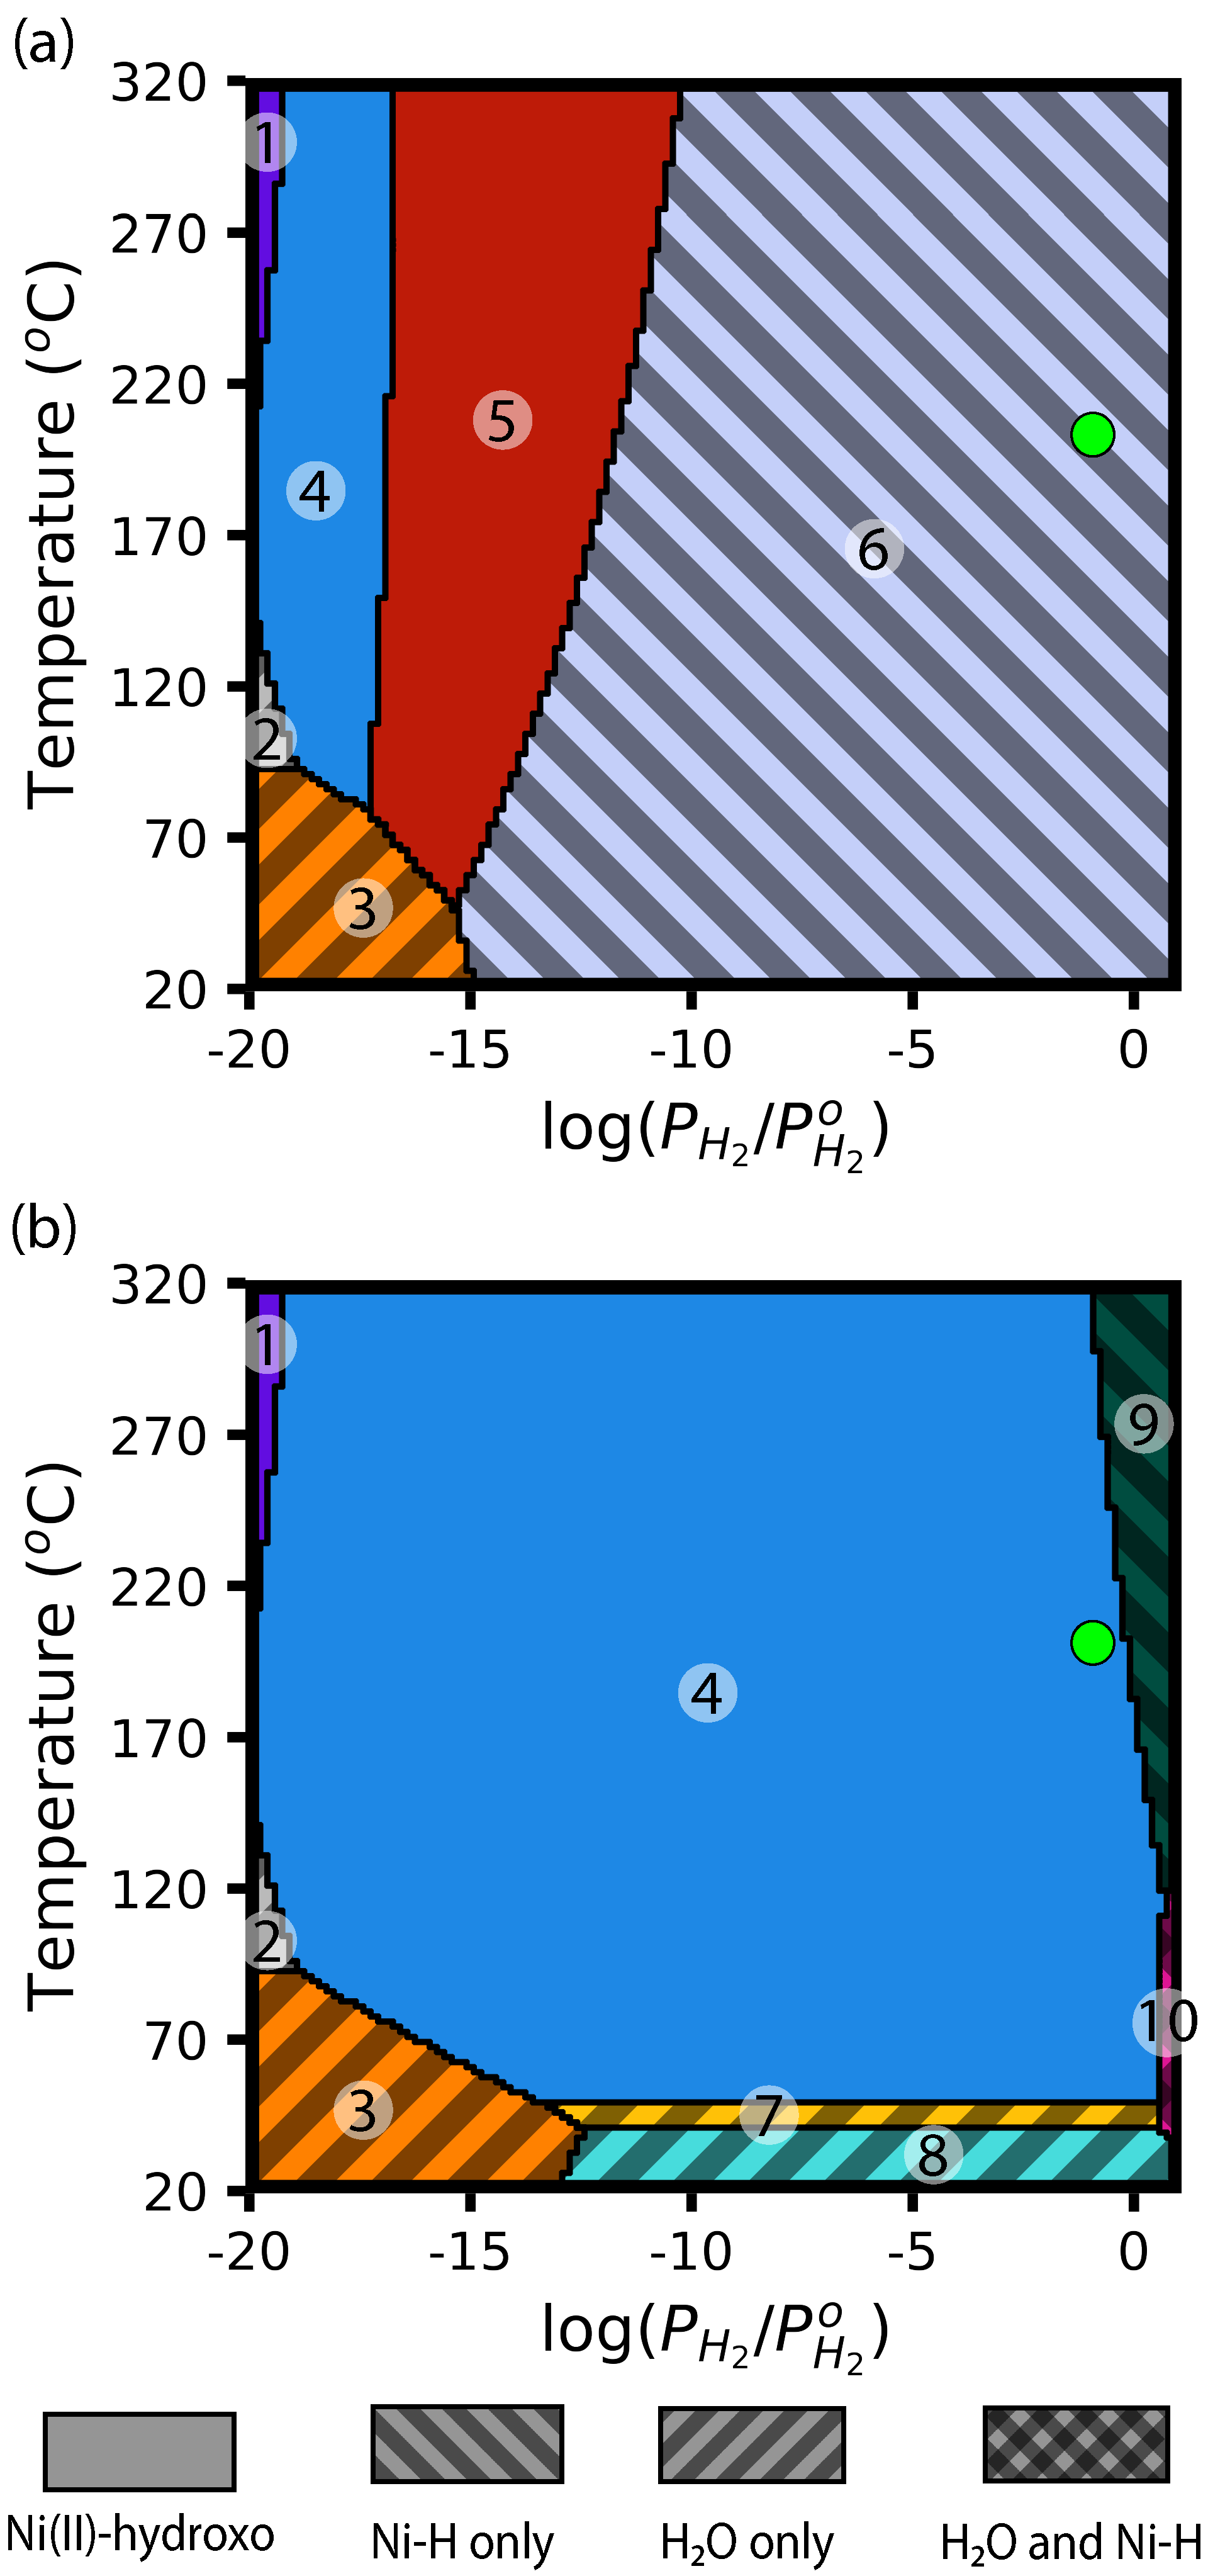
\includegraphics{zi-images/01-Ni-Graphics/2021-MAIN-phase-diagram-combined.png}
    \caption{
    Phase diagrams for the Ni cluster catalyst calculated at $P_{\ce{H2O}}=10^{-1}$ bar as a function of $T$ and $P_{\ce{H}_2}$ with (a) variable \ce{Ni} composition and (b) fixed \ce{Ni} composition (\ce{Ni}=4). The different structures are represented by the different colored and numbered regions; the color and numbering schemes are the same as in Figures~\ref{fig:Ni-structure-diagram} and \ref{fig:dPDFs_TandP_trans_Ni}. In (a), the \ce{Ni} chemical potential ($\mu_{\ce{Ni(s)}} \approx E_{\ce{Ni(s)}}$), whereas in (b) the number of \ce{Ni} atoms ($N_{\ce{Ni(s)}}=4$) is fixed. The green dot represents $T$ and $P_{\text{\ce{H2}}}$ conditions observed experimentally.
    }
    \label{fig:phase_diagram_Ni_combined}
\end{figure}  

% Structure Diagram
\begin{figure}[H]
    \centering
    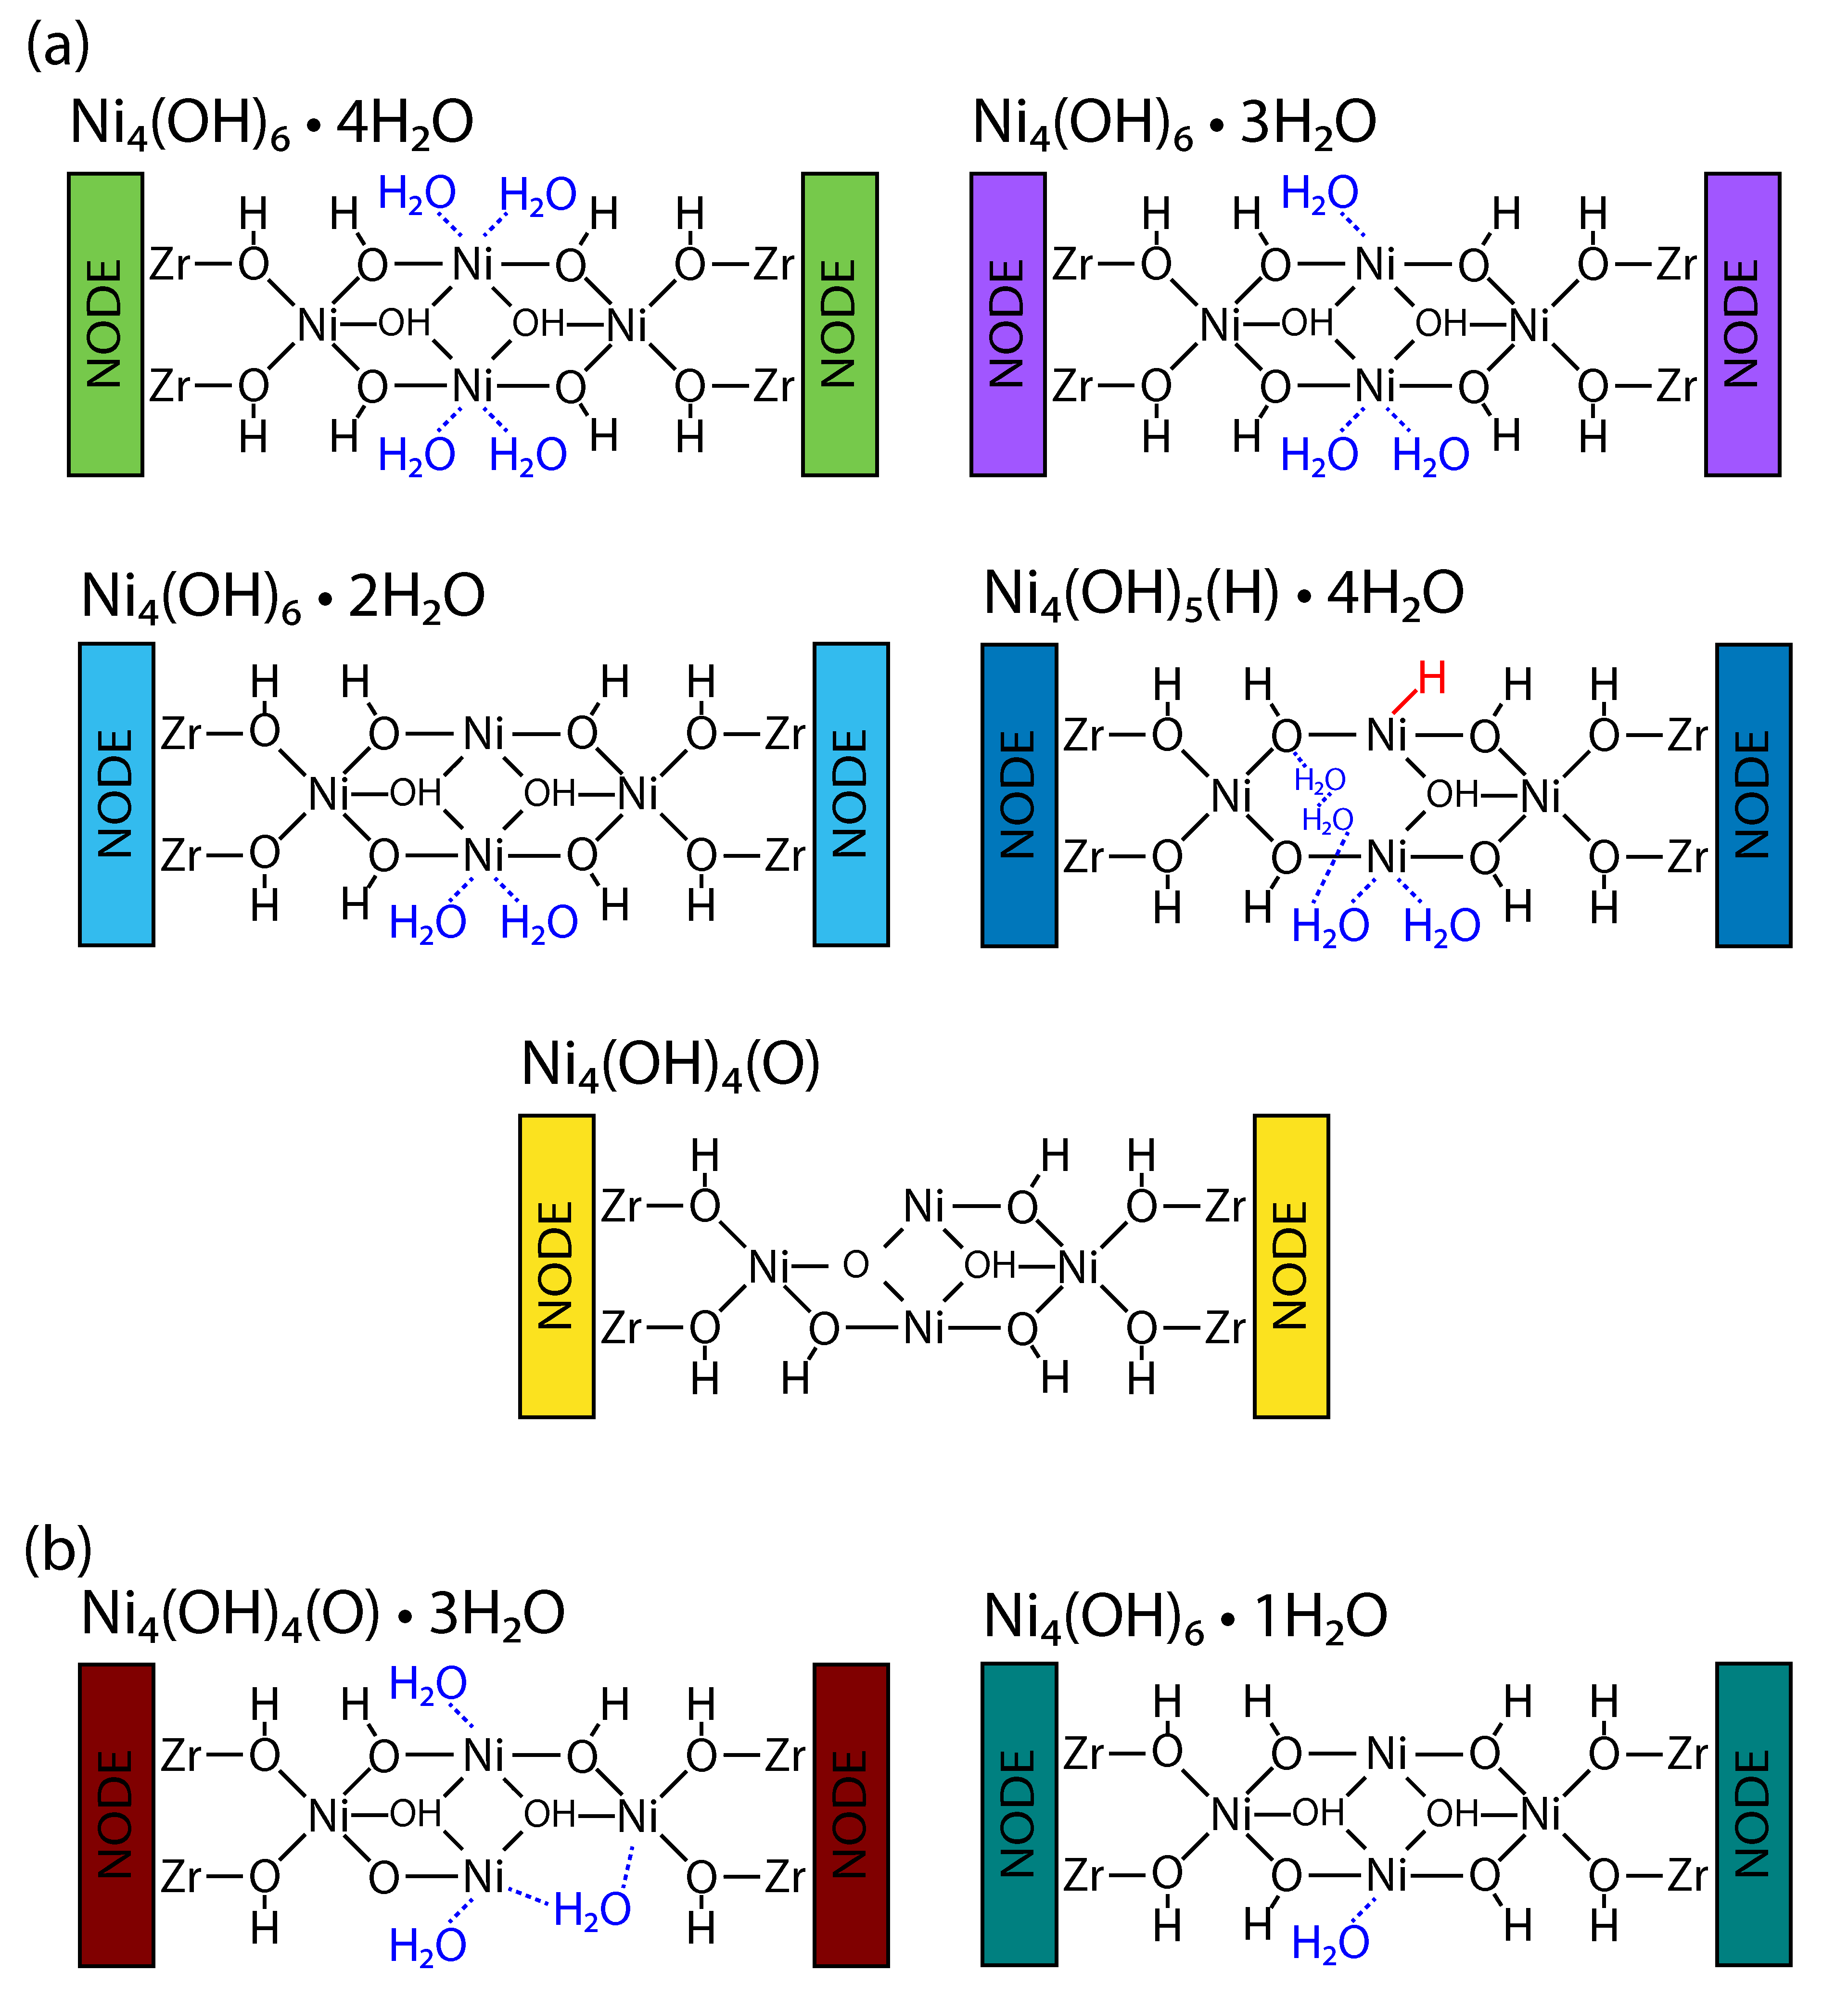
\includegraphics{zi-images/01-Ni-Graphics/2021-MAIN-structure-diagram.png}
    \caption{
    Depictions of key structures considered in this work along with the names used to identify them. The color and numbering schemes are the same as in Figures~\ref{fig:phase_diagram_Ni_combined} and \ref{fig:dPDFs_TandP_trans_Ni}. Structure denoted with an $\blacklozenge$ are not thermodynamic minimum under any of the explored conditions. All \ce{H2O}s within the structure are colored blue, and any Nickel hydride species (\ce{Ni-H}) are colored red.
    }
    \label{fig:Ni-structure-diagram}
\end{figure}

%The local coordination of the \ce{Ni} atoms vary significantly as a function of the environmental conditions (Figure~\ref{fig:Ni-structure-diagram}). 
%Given the discrepancies in coordination numbers and dPDFs for structures featuring variable \ce{Ni} content, we shift our focus towards structures with a a fixed \ce{Ni} composition of four (Figure~\ref{fig:phase_diagram_Ni_combined} (b)).

To provide further insight into the structure and composition of the Ni catalyst, dPDFs for structures 1, 3, 4, 5, 6, 7, and 8 (purple, orange, blue, red, and lilac lines), i.e., those that ... state rational for including these in the dPDF figure, are compared with the dPDF from the experimental structure (black line) is provided in Figure~\ref{fig:dPDFs_TandP_trans_Ni}. Key peaks in the experimentally observed dPDF are the single peak at 2.02 {\AA}, split peaks at 3.01 {\AA} and 3.27 {\AA}, and split peaks at 3.78 {\AA} and 4.08 {\AA}. These correspond to \ce{Ni-O}, \ce{Ni{\Compactcdots}Ni}, and \ce{Ni{\Compactcdots}Zr} distances, respectively. 

The presence of five peaks suggests a Ni coordination number of ca. 5. This rules out structures 4-\ce{Ni4(OH)4} (light blue), 5-\ce{Ni3(OH)2} (red), 6-\ce{Ni2(H)2} (lilac), and 7-\ce{Ni4(OH)4.H2O} (yellow), which all have Ni coordination numbers less than 5. Notably, structures with fewer than four Ni cations (i.e., most of the structures on Figure 2b) cannot achieve such high coordination. As removal of \ce{Ni} occurs via the removal of $\ce{OH^{*}}$ ligands, the presence of $\ce{OH^{*}}$ ligands is vital in keeping the structure together. Structures that contain \ce{Ni} atoms featuring high coordination with either $\ce{OH^{*}}$ or $\ce{H2O^{*}}$ ligands show better agreement with the experimental dPDF (Figure~\ref{fig:dPDFs_TandP_trans_Ni}). 

In general, the simulated structures give good agreement with the \ce{Ni-O} peak compared to the experimental peak, with the following exceptions. Additionally, structures xxx exhibit broadening (skewed right) of the \ce{Ni-O} peak for a few structure, suggesting xxx. 

The split peaks in the experimental dPDF at 3.01 {\AA} and 3.27 {\AA} suggest asymmetry in the Ni coordination environments. Most structures appearing on the phase diagram (Figure~\ref{fig:phase_diagram_Ni_combined}) are symmetric in their ligand coordination (as showed by the structures located in Figure~\ref{fig:Ni-structure-diagram}). When inspecting the interatomic distances, the distances tend to be symmetric thereby leading to single peaks \ce{Ni{\Compactcdots}Ni} instead of multiple \ce{Ni{\Compactcdots}Ni} in the 3.01 {\AA} and 3.27 {\AA} range. The exception is structure 8-\ce{Ni4(OH)5(H).4H2O}, which comprises OH, H2O, and H ligands in the first coordination spheres. Notably, this structure also features a hydrogen bonded chain of H2O molecules that spans from one Ni to an OH ligand on the other side of the cluster. This asymmetric ligand environment breaks the symmetry of coordination, leading to the split to the split \ce{Ni{\Compactcdots}Ni} peaks at distances that closely reasonable those seen in the experimental dPDFs.  

Further evidence for highly coordinated Ni is observed from the Ni-Ni peaks. As the structures are reduced (\ce{Ni} atoms become uncoordinated), we start to observe the presence of a \ce{Ni{\Compactcdots}Ni} peak around 2.3 {\AA} which has a distance shorter than the bond of converged bulk \ce{Ni} (2.46 {\AA}). Additionally, we observe a lack of \ce{Ni{\Compactcdots}Ni} peak split around the 3.01 {\AA} and 3.27 {\AA} peaks shown by the experimental dPDF.

The last remaining feature of the dPDFs not explored are the \ce{Ni{\Compactcdots}Zr} split peaks seen in the 3.78 {\AA} and 4.08 {\AA} range in the experimental dPDF (Figure~\ref{fig:dPDFs_TandP_trans_Ni}). Similar to the \ce{Ni{\Compactcdots}Ni} split peaks, most structures exhibit a single peak within the experimental range. Of the structures in the phase diagram, only 7-\ce{Ni4(OH)4.H2O} (yellow) shows splitting of the \ce{Ni{\Compactcdots}Zr} peaks. Any explanation for why 7 shows this peak splitting? The \ce{Ni{\Compactcdots}Zr} distance within the MOF is from the attachment of the Nickel SSHC to the MOF node. The \ce{Ni} atoms are connected to the \ce{Zr} via \ce{OH} ligands within our model, so single peaks suggests that distances between the two \ce{Ni} and \ce{Zr} atoms are uniform. To exhibit asymmetry, we expect that either the two \ce{Ni} ions that connect to the \ce{Zr} nodes will have coordination environments that differ from each other or that the NU-1000 unit cell exhibits asymmetry around the c pore under reaction conditions. For example, the experimentally observed \ce{Ni{\Compactcdots}Zr} split peaks could be caused by node distortions (i.e., deformations in the MOF crystalline structure). As presently formulated, our model fails to consider any deformations of the MOF crystalline structure. Our unit cell parameters are fixed throughout the entire simulation. As the unit cell dimensions and shapes are held fixed in our models, our models are better able to capture asymmetry due to different ligand environments but not due to structural effects. Possible deviations include different coordinating ligands between the two atoms, such as was explored by \citeauthor{Shabbir2020} on a single atom Nickel catalyst.\cite{Shabbir2020}  We did consider variations to the ligands that coordinate directly to the MOF node (\ce{Zr}) and the Nickel SSHC (\ce{Ni}). However, these structures were not thermodynamic minima under any of the explored conditions.  

% Our models comprising four Ni ions contain two types of \ce{Ni} ions: two that connect to the \ce{Zr} nodes and two that do not (e.g., see Figures~\ref{fig:Ni-MOF-model} (c), \ref{fig:Ni-MOF-model} (d), and \ref{fig:Ni-structure-diagram}). 

% tructures 5-\ce{Ni3(OH)2} (red) and 6-\ce{Ni2(H)2} (lilac) represent the two structures on the phase diagram (Figure~\ref{fig:phase_diagram_Ni_combined} (a)) with Nickel contents less than four and several $\ce{OH^{*}}$ ligands removed. The dPDFs shows an underprediction in the \ce{Ni-O} peak, with 5-\ce{Ni3(OH)2} (red) overpredicting the \ce{Ni{\Compactcdots}Ni} peaks and 6-\ce{Ni2(H)2} not including any \ce{Ni{\Compactcdots}Ni} peaks (as described by Figure~\ref{fig:dPDFs_TandP_trans_Ni}).

%Based on the modeling, we suggest that the presence of a direct \ce{Ni-Ni} bond is not seen experimentally and that again we expect a high local coordination involving both \ce{OH} or \ce{H2O} ligands. The structures that meet these criteria show better agreement to the experimental dPDFs with the bulk of these structure observed at lower \ce{H2} partial pressures. However, we do not find a structure that contains perfect agreement with the experimental dPDF.

%Also of interest is that the dominant structure in Figure~\ref{fig:phase_diagram_Ni_combined} (b) is structure 4-\ce{Ni4(OH)4} (light blue), which consists of four \ce{Ni} atoms linked together by four \ce{\mu-OH} ligands. The ligand environment of 4-\ce{Ni4(OH)4} (light blue) is similar to the model from \citeauthor{Ye2017}, which when exposed to a different set of environment conditions generated coordinated \ce{H}, \ce{C2H4}, \ce{C2H5} to the middle \ce{Ni} atoms.\cite{Ye2017}

% We determined the binding energy of the \ce{H2O} molecule that is uncoordinated to any cluster \ce{Ni} atoms in the chain is -104 kJ/mol, which is lower in energy than \ce{H2O} coordinated to \ce{Ni} (~-75 kJ/mol). The more favorable binding energy suggests that despite not being coordinated to any \ce{Ni}, that the \ce{H2O} has favorable interactions with other parts of the MOF (i.e., the node or the pyrene linker). The distance between a carbon atom in pyrene-linker and the \ce{H} atom (in the \ce{H2O} molecule) is 2.37 {\AA} and 2.70 {\AA}, respectively.

% This difference between experiments and simulations could be due to kinetics or other things not included in the models.

% dPDF diagram for the phase diagram structures 
\begin{figure}[H]
    \centering
    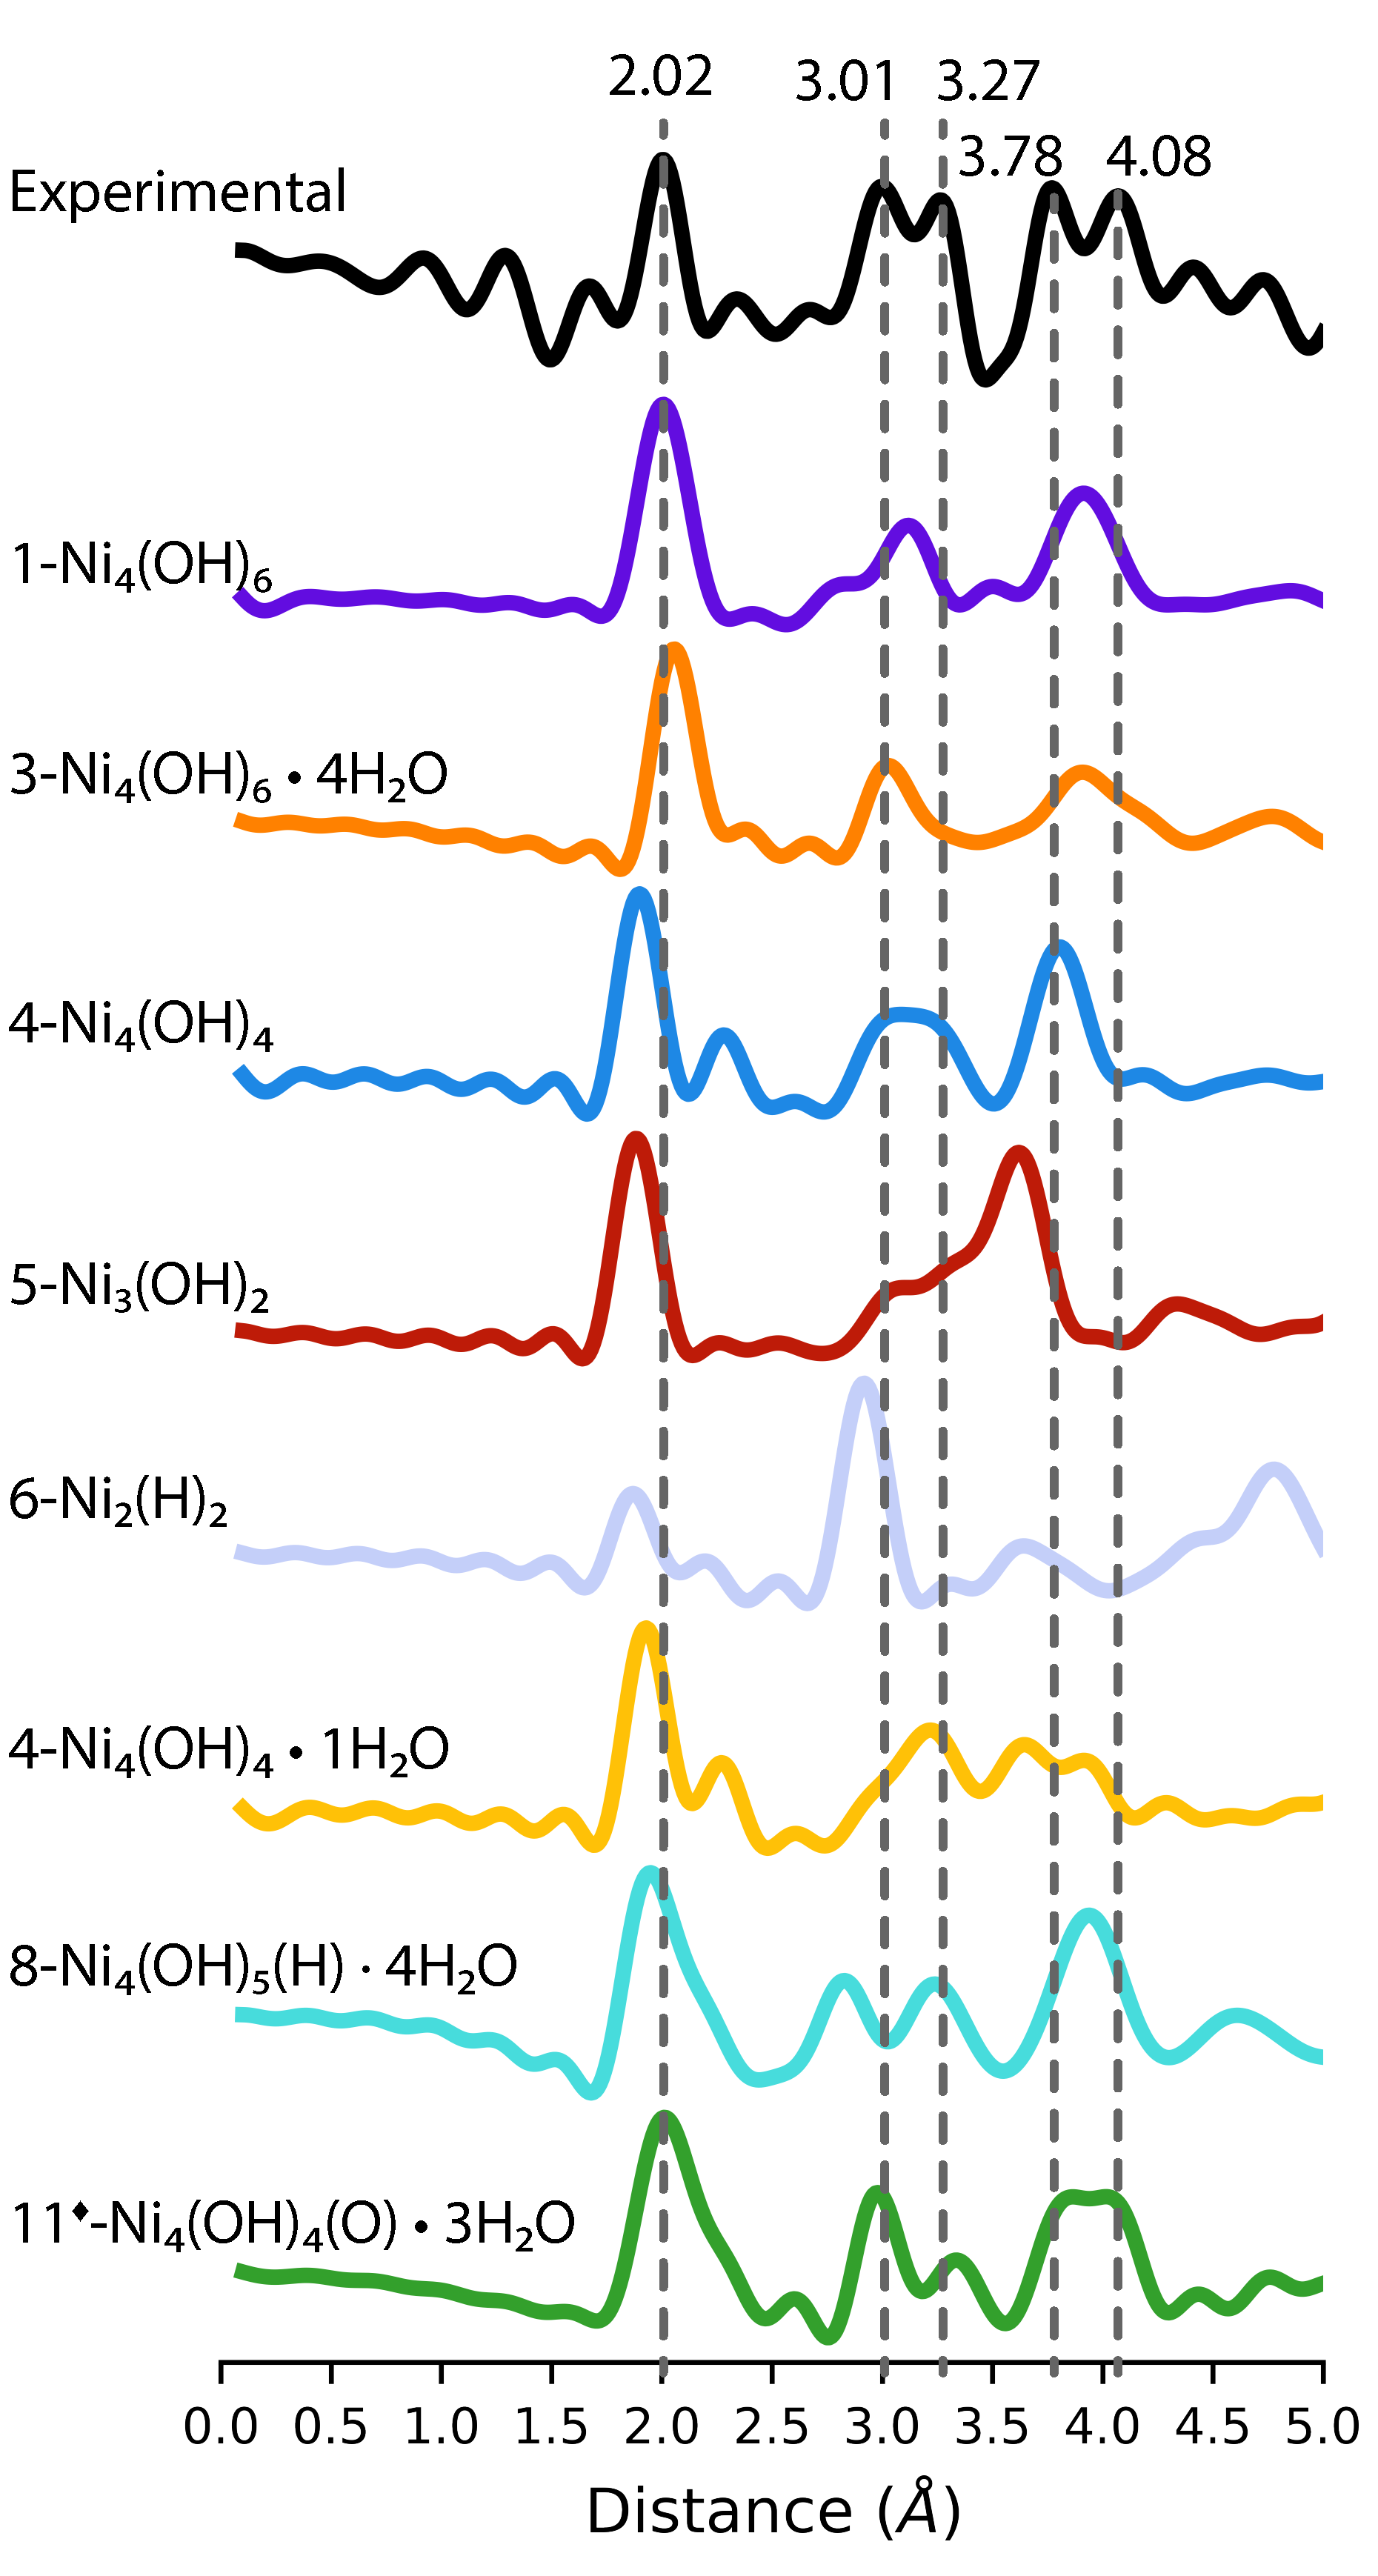
\includegraphics{zi-images/01-Ni-Graphics/2021-MAIN-single-dPDF-highH2O.png}
    \caption{
    Differential pair distribution functions (dPDFs) for experimental and simulated structures considered in this study. The color and numbering schemes are the same as in Figures~\ref{fig:phase_diagram_Ni_combined} and \ref{fig:Ni-structure-diagram}.  
    }
    \label{fig:dPDFs_TandP_trans_Ni}
\end{figure}

%Of interest is the catalyst composition and structure under operating conditions, i.e., 0.05~bar \ce{H2} and $T \le$~200~K, signified by the green dot on each phase diagram (Figure~\ref{fig:phase_diagram_Ni_combined}). The structure that minimizes $F^{(3)}$ at these conditions, according to Figure~\ref{fig:phase_diagram_Ni_combined} (a), i.e., where the compositions of hydride, hydroxyl, and water ligands as well as \ce{Ni} atoms are allowed to vary, is 6-\ce{Ni2(H)2} (lilac) (from Figure~\ref{fig:Ni-structure-diagram}). This structure features two isolated single \ce{Ni} ion hydride structures, similar to models used in prior catalytic studies.\cite{Li2016sintering,Shabbir2020,Hackler2020} However, the dPDF for this structure is in stark contrast with the experimental dPDF, given its low \ce{Ni} coordination number of ca. 3. Further, the dPDF for structure 6-\ce{Ni2(H)2} (lilac) does not match well with the experimentally observed one. In fact, given that removal of \ce{Ni} only occurs after significant depletion of $\ce{OH^{*}}$, which in turn decreases the Ni coordination number, the only structures from our library that have the possibility of matching the experimental dPDF are those with four Ni ions. Hence, Figure~\ref{fig:phase_diagram_Ni_combined} (b) provides a phase diagram where the number of \ce{Ni} atoms is held fixed at 4.

%While several structures on this phase diagram exhibit \ce{Ni-O} peaks in good agreement with experiment, only one, 8-\ce{Ni4(OH)5(H).4H2O} (teal in Figure~\ref{fig:Ni-structure-diagram}), exhibits double \ce{Ni{\Compactcdots}Ni} peaks. This ``teal" structure features hydride ($\ce{H^{*}}$), hydroxyl ($\ce{OH^{*}}$), and water ($\ce{H2O^{*}}$) ligands as well as additional \ce{H2O} molecules that form a hydrogen bonded chain between a hydroxyl ligand and a water ligand. \st{and is the thermodynamically preferred structure under conditions of relevance to catalysis}. 
   

 

%%%%%%%%%%%%%%%%%%%%%%%%%%%%%%%%%%%%%%%%%%%%%%%%%%%%%%%%%%%%%%%%%%%%%
%% Discussion
%%%%%%%%%%%%%%%%%%%%%%%%%%%%%%%%%%%%%%%%%%%%%%%%%%%%%%%%%%%%%%%%%%%%

\section{Discussion}

Of the structures represented in Figures 2a and 2b, only 7 and 8 exhibit peak splitting observed experimentally. While these structures capture double peaks for the \ce{Ni{\Compactcdots}Ni} (8) or \ce{Ni{\Compactcdots}Zr} (7) distances, they are still not a good match with experiment, as they comprise Ni with coordination number smaller than 5 (7) or broaden the Ni-O peak (8) and underpredict the \ce{Ni-O} distance (7 and 8). Further, these structures contains a single \ce{Ni{\Compactcdots}Ni} (7) or \ce{Ni{\Compactcdots}Zr} (8) peak. Hence, to provide further insight into the ligand composition of the observed structure, we searched our structural database for structures that more closely matched the experimental dPDF. The structure from our library that gave the best agreement with the experimental dPDFs is 11$^{\blacklozenge}$-\ce{Ni4(OH)4(O).3H2O} (green), shown in Figures 3 and 4. It should be noted that this structure is not a thermodynamic minimum, according to our analysis, which is why it does not appear on the phase diagram. This structure comprises hydride, hydroxyl, and water ligands and additionally includes a \ce{\mu_{2}-O} ligand instead of a \ce{\mu_{2}-OH} ligand. The composition of structure 11$^{\blacklozenge}$-\ce{Ni4(OH)4(O).3H2O} (green) is both compositional diverse and asymmetric with ligand coordination. The structure contains $\ce{OH^{*}}$, $\ce{H2O^{*}}$, and even a $\ce{O^{*}}$ ligand. The \ce{Ni} coordination is such that the $\ce{OH^{*}}$ and $\ce{O^{*}}$ link adjacent two \ce{Ni} atoms. Additionally, an $\ce{H2O^{*}}$ ligand occupies the space of a $\ce{OH^{*}}$ ligand (i.e., the $\ce{H2O^{*}}$ ligand is coordinated to two \ce{Ni} atoms). The structure features high \ce{Ni} coordination, which as previously discussed, is an important characteristic of structures resemble the experimental structure. From Figure~\ref{fig:dPDFs_TandP_trans_Ni}), the dPDF for 11$^{\blacklozenge}$-\ce{Ni4(OH)4(O).3H2O} (green) shows good agreement for the \ce{Ni-O} peak when compared to the experimental dPDF. Additionally, 11$^{\blacklozenge}$-\ce{Ni4(OH)4(O).3H2O} (green) contains split \ce{Ni{\Compactcdots}Ni} peaks that closely matched the experimental dPDF. For the split \ce{Ni{\Compactcdots}Ni} peaks, 11$^{\blacklozenge}$-\ce{Ni4(OH)4(O).3H2O} shows the best agreement compared to the experimental dPDF. Given that the structure dPDF that best agrees with the experimental dPDF contains the compositional diverse ($\ce{OH^{*}}$, $\ce{H2O^{*}}$, and $\ce{O^{*}}$ ligands) and asymmetric ($\ce{H2O^{*}}$ occupying a `defect' site and $\ce{O^{*}}$ ligand coordinating two \ce{Ni} atoms) ligand coordination suggests that considering alternative structures is important. Although not as pronounced, the green structure also exhibits \ce{Ni{\Compactcdots}Zr} peak splitting. While this structure still does not reproduce the experimental dPDF, it provides clues as to the composition and structure of the Ni cluster under catalytic operating conditions. Specifically, this structure is likely to comprise at least four Ni ions with high coordination that involves diverse ligand coordination. 

% Although 11$^{\blacklozenge}$-\ce{Ni4(OH)4(O).3H2O} (green) doesn't appear on the phase diagram (Figure~\ref{fig:phase_diagram_Ni_combined}), our analysis still suggests that a diverse ligand coordination is present as a result of environmental conditions.

%Within our modeling efforts, we also performed dPDF analysis on structures that were not local minima and thus were not considered in the phase diagrams (Figure~\ref{fig:phase_diagram_Ni_combined}). Structure that aren't local minima (lowest energy) at their specific compositions were not considered during \textit{ab initio} thermodynamic analysis. Only structures that are local minima at their specific compositions could appear on the phase diagram (Figure~\ref{fig:phase_diagram_Ni_combined}). However, we searched the library of structures to identify compositions that demonstrate features resembling the \ce{Ni-O} and \ce{Ni{\Compactcdots}Ni} peaks. One such structure is 11$^{\blacklozenge}$-\ce{Ni4(OH)4(O).3H2O} (green), as seen in Figure~\ref{fig:Ni-structure-diagram} and \hl{Figure SXXX}.  

%Third, our modeling efforts directly demonstrate why consideration of environmental conditions on SSHCs are vital. Figure~\ref{fig:phase_diagram_Ni_combined} provides direct evidence at the structurally diversity of the ligand coordination environment as a function of the environmental conditions for a Nickel metal complex supported on a MOF while considering environmental conditions. 

% Therefore, any structures exhibiting a \ce{Ni{\Compactcdots}Zr} split peak within the 3.78 {\AA} and 4.08 {\AA} range are encouraging; however, we do not evaluate structural performance based on a structures ability to demonstrate \ce{Ni{\Compactcdots}Zr} split peaks.

\section{Conclusions}
We present the rich structural landscape of a \ce{Ni} metal complex using a combination of \textit{ab initio} thermodynamic analysis, which combines density functional theory (DFT) and empirical gas phase thermochemistry to determine the thermodynamic stability of a \ce{Ni} metal complex at different conditions, and dPDF. We explore the influence of temperature, \ce{H2O} partial pressure, and \ce{H2} partial pressure on the thermodynamic stability and report our finding as phase diagrams. We quantify the local structures of our model using dPDF analysis, and compare our model structures to experimental dPDF for a \ce{Ni} metal complex supported on NU-1000. Comparisons with experiments reveal the importance of a high \ce{Ni} coordination environment, which is maintained by coordinated \ce{OH} and \ce{H2O} groups to the \ce{Ni} atoms of the cluster. When exposed to \ce{H2} and elevated temperatures, our model shows the removal of \ce{OH} ligands, resulting in lower \ce{Ni} coordination within the active site. Structures with a low \ce{Ni} coordination generate peaks that are not observed experimentally. With a higher \ce{H2O} partial pressure, our \textit{ab initio} thermodynamic modeling produce structures that include both \ce{OH} and \ce{H2O} species within the active site. We expand from structures that are thermodynamic minima to include other structures within the library. A general trend is that the structures containing more \ce{OH} and \ce{H2O} groups show better agreement to the experimental dPDF in our dPDF analysis, and these structures become thermodynamically relevant at higher \ce{H2O} partial pressures. 

Interestingly, only few of the structures on Figure \ref{fig:phase_diagram_Ni_combined} comprise hydride (\ce{Ni-H}), which have been previously suggested as the active site in hydrogenation catalysis.\cite{Li2016sintering,Shabbir2020} Note that the previous work by \citeauthor{Li2016sintering} and \citeauthor{Shabbir2020} consisted of a single \ce{Ni} atoms coordinate to the MOF node. Upon exposure to \ce{H2} gas, the Nickel SSHC is thought to dissociate molecular \ce{H2} into atomic \ce{H} with a \ce{Ni-H} forming and the additional \ce{H} atom being adsorbed by one of the $\ce{OH^{*}}$ ligands. We explored structures using a similar approach and systematically generated the structures to include $\ce{H^{*}}$ (thus forming the \ce{Ni-H} species). Structures containing a \ce{Ni-H} were included in \textit{ab initio} thermodynamic analysis, but only structures  6-\ce{Ni2(H)2} (lilac) and 8-\ce{Ni4(OH)5(H).4H2O} contain a \ce{Ni-H} with neither structure showing reasonable agreement with the experimental dPDF (Figure~\ref{fig:dPDFs_TandP_trans_Ni}). While this work does not rule out metal hydrides as active sites, it suggests that other ligands, e.g., $\ce{OH^{*}}$ or $\ce{H2O^{*}}$ ligands, could participate in the active site for catalysis. The proton ($\ce{H^{*}}$) necessary for hydrogenation could come from either the $\ce{OH^{*}}$ or $\ce{H2O^{*}}$ ligands with exposure to \ce{H2} gas regenerating these ligands. The lack of \ce{Ni-H} raises questions about the catalytically active group for the \ce{Ni} metal complex catalyst. 

Overall, the findings establish improve models that require further computational catalytic investigations, including the exploration of the kinetic barriers related to these transformations.
 
\section{References}

%The class makes various changes to the way that references are
%handled.  The class loads \textsf{natbib}, and also the
%appropriate bibliography style.  References can be made using
%the normal method; the citation should be placed before any
%punctuation, as the class will move it if using a superscript
%citation style
%\cite{Mena2000,Abernethy2003,Friedman-Hill2003,EuropeanCommission2008}.
%The use of \textsf{natbib} allows the use of the various citation
%commands of that package: \citeauthor{Abernethy2003} have shown
%something, in \citeyear{Cotton1999}, or as given by
%Ref.~\citenum{Mena2000}.  Long lists of authors will be
%automatically truncated in most article formats, but not in
%supplementary information or reviews \cite{Pople2003}. If you
%encounter problems with the citation macros, please check that
%your copy of \textsf{natbib} is up to date. The demonstration
%database file \texttt{achemso-demo.bib} shows how to complete
%entries correctly. Notice that ``\latin{et al.}'' is auto-formatted
%using the \texttt{\textbackslash latin} command.

%Multiple citations to be combined into a list can be %given as
%a single citation.  This uses the \textsf{mciteplus} %package
%\cite{Johnson1972,*Arduengo1992,*Eisenstein2005,*Arduengo%1994}.
%Citations other than the first of the list should be %indicated
%with a star. If the \textsf{mciteplus} package is not %installed,
%the standard bibliography tools will still work but %starred
%references will be ignored. Individual references can be %referred
%to using \texttt{\textbackslash mciteSubRef}:
%``ref.~\mciteSubRef{Eisenstein2005}''.

%The class also handles notes to be added to the bibliography.  These
%should be given in place in the document \bibnote{This is a note.
%The text will be moved the the references section.  The title of the
%section will change to ``Notes and References''.}.  As with
%citations, the text should be placed before punctuation.  A note is
%also generated if a citation has an optional note.  This assumes that
%the whole work has already been cited: odd numbering will result if
%this is not the case \cite[p.~1]{Cotton1999}.

%%%%%%%%%%%%%%%%%%%%%%%%%%%%%%%%%%%%%%%%%%%%%%%%%%%%%%%%%%%%%%%%%%%%%
%% The "Acknowledgement" section can be given in all manuscript
%% classes.  This should be given within the "acknowledgement"
%% environment, which will make the correct section or running title.
%%%%%%%%%%%%%%%%%%%%%%%%%%%%%%%%%%%%%%%%%%%%%%%%%%%%%%%%%%%%%%%%%%%%%
%\begin{acknowledgement}
%
%\hl{authors would like to thank \ldots''.
%
%The author thanks Mats Dahlgren for version one of \textsf{achemso},
%and Donald Arseneau for the code taken from \textsf{cite} to move
%citations after punctuation. Many users have provided feedback on the
%class, which is reflected in all of the different demonstrations
%shown in this document.}
%
%\end{acknowledgement}

%%%%%%%%%%%%%%%%%%%%%%%%%%%%%%%%%%%%%%%%%%%%%%%%%%%%%%%%%%%%%%%%%%%%%
%% The same is true for Supporting Information, which should use the
%% suppinfo environment.
%%%%%%%%%%%%%%%%%%%%%%%%%%%%%%%%%%%%%%%%%%%%%%%%%%%%%%%%%%%%%%%%%%%%%
%\begin{suppinfo}
%
%\hl{This will usually read something like: ``Experimental procedures and
%characterization data for all new compounds. The class will
%automatically add a sentence pointing to the information on-line:}
%
%\end{suppinfo}

%%%%%%%%%%%%%%%%%%%%%%%%%%%%%%%%%%%%%%%%%%%%%%%%%%%%%%%%%%%%%%%%%%%%%
%% The appropriate \bibliography command should be placed here.
%% Notice that the class file automatically sets \bibliographystyle
%% and also names the section correctly.
%%%%%%%%%%%%%%%%%%%%%%%%%%%%%%%%%%%%%%%%%%%%%%%%%%%%%%%%%%%%%%%%%%%%%
\bibliography{achemso-demo}

\end{document}